%%%%%%%%%%%%%%%%%%%%%%%%%%%%%%%%%%%%%%%%%%%%%%%%%%%%%%%%%%%%%%%%%%%%%%%%%%%%%%%%%%
\begin{frame}[fragile]\frametitle{}
\begin{center}
{\Large Notes from Samkhya Darshan}
\end{center}
\end{frame}

%%%%%%%%%%%%%%%%%%%%%%%%%%%%%%%%%%%%%%%%%%%%%%%%%%%%%%%%%%%%%%%%%%%%%%%%%%%%%%%%%%
\begin{frame}[fragile]\frametitle{Background}

      \begin{itemize}
        \item मनुष्य की हमेशा से जिज्ञासा रही है की हमारा अस्तित्व आया कहां से? हमारे अतीत का कारण क्या है? ब्रह्मांड की उत्पत्ति हुई कहां से? जो हमारी ऋषि मुनि हुए उनको भी यह सब समझना था 
		\item  ढेर सारे मजहब बताते हैं की सृष्टि को किसी ईश्वर ने बना दिया है. इस धार्मिक विचार से हटकर हमारे ऋषि मुनियों ने दी  और जो बहुत तार्किक को शास्त्रीय हो, वो है, सांख्य दर्शन 
		\item सनातन धर्म के केंद्र में जो चार वेद है ऋग्वेद यजुर्वेद सामवेद अथर्ववेद और उनके भाग, आरण्यक, ब्राह्मण , संहिता ,  उपनिषद.  इनके आधार पर जब ऋषि मुनियों ने अध्ययन किया तो छह दर्शन मानव जीवन को समझने के लिए दिये, उसमेसे एक है सांख्य दर्शन 
		\item इनमें किसी में कर्म को ऊपर रखा गया है किसी में भक्ति के ऊपर रखा गया है किसी में ज्ञान को ऊपर रखा गया क्योंकि यही तीन
माध्यम है जो सनातन धर्म में ईश्वर को ईश्वर तक पहुंचने के लिए बताए गए हैं की कर्म ज्ञान और भक्ति तीन तरह के रास्ते हैं.
		\item यह एक दूसरे से काफी अलग है इनमें से कुछ दर्शन बहुईश्वरवाद को मानती हैं कुछ एक भगवान को मानते हैं, और कुछ
भगवान को मानती नहीं है 
\item यह संख्या दर्शन है वह भी अनीश्वरवादी  (agnostic) है वह ईश्वर को भले  न नाकारती हो लेकिन यह भी नहीं मानती ईश्वर सृष्टि की रचना किए होंगे कोई मतलब ऐसे बाहर से कुछ धक्का  दे के  ब्रह्मांड बना हो
      \end{itemize}



\end{frame}



%%%%%%%%%%%%%%%%%%%%%%%%%%%%%%%%%%%%%%%%%%%%%%%%%%%%%%%%%%%%%%%%%%%%%%%%%%%%%%%%%%
\begin{frame}[fragile]\frametitle{सांख्य दर्शन की भूमिका (Introduction to Sāṅkhya Darśana)}
\begin{columns}
    \begin{column}[T]{0.6\linewidth}
      \begin{itemize}
        \item "सांख्य" का अर्थ – क्रमबद्ध विवेचन (rational enumeration), तार्किक, विश्लेषणात्मक और वैज्ञानिक दृष्टिकोण
        \item दर्शन is a proposed mental model to explain the origin of the universe as well as how it runs!!		
        \item कपिल मुनि (Kapila Muni)   प्रवर्तक , 700 BC
        \item \textbf{अनीश्वरवादी} (Anīśvaravādī, Agnostic), ईश्वर को सृष्टिकर्ता नहीं मानता
        \item फिर भी यह \textbf{आस्तिक} (Āstika) दर्शन है,  वेदों को प्रमाण मानता है
        \item गीता, भागवत, महाभारत में इसके तत्वों का उल्लेख
        \item बौद्ध (नास्तिक) और आस्तिक परंपराओं दोनों पर इसका प्रभाव
		\item बुद्ध ने अपना बचपन कपिलवस्तु नाम की नगरी पर उन्होंने बिताया है 

      \end{itemize}
    \end{column}
    \begin{column}[T]{0.4\linewidth}
      \begin{center}
        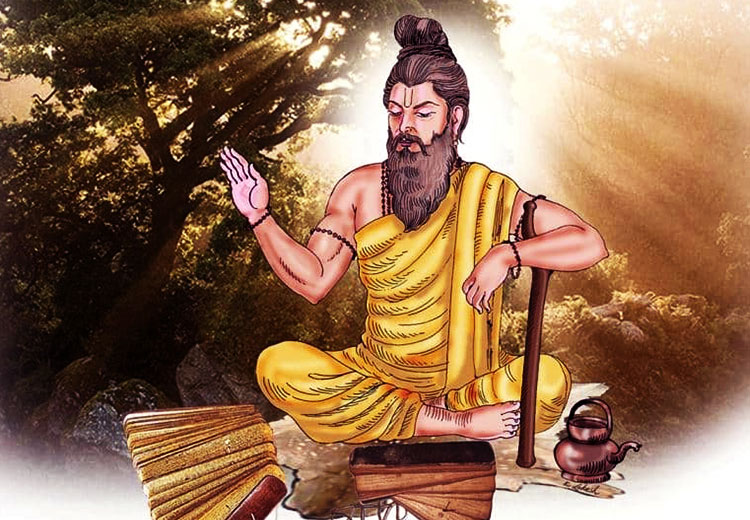
\includegraphics[width=\linewidth,keepaspectratio]{sankhya1}
		
        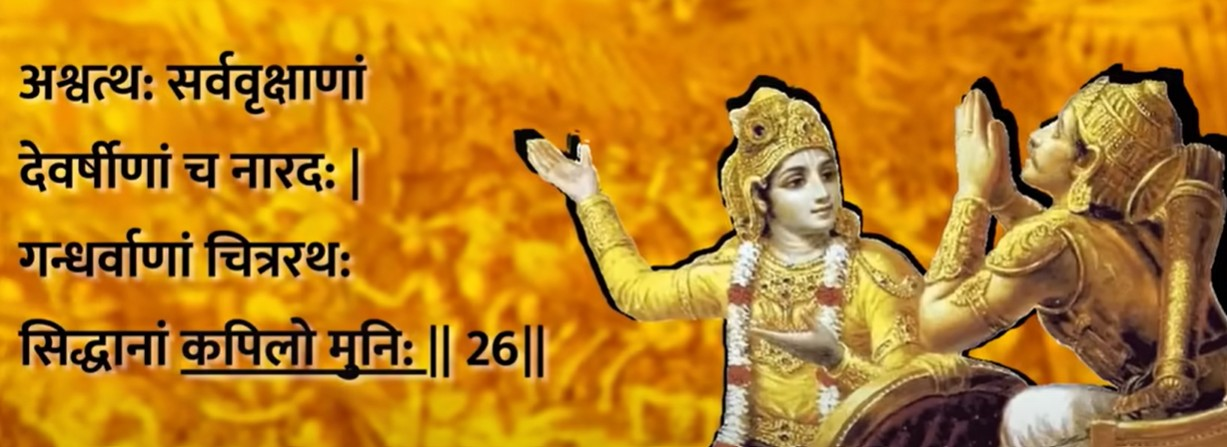
\includegraphics[width=\linewidth,keepaspectratio]{sankhya2}
		
		{\tiny (Ref: Samkhya Darshan - HyperQuest)}
		
      \end{center}	
    \end{column}
\end{columns}
\end{frame}

%%%%%%%%%%%%%%%%%%%%%%%%%%%%%%%%%%%%%%%%%%%%%%%%%%%%%%%%%%%%%%%%%%%%%%%%%%%%%%%%%%
\begin{frame}[fragile]\frametitle{मुख्य ग्रंथ (Principal Texts)}
\begin{columns}
    \begin{column}[T]{0.6\linewidth}
      \begin{itemize}
        \item मूल ग्रंथ: \textbf{सांख्य प्रवचन सूत्र (Sāṅkhya Pravacana Sūtra)} कपिल मुनि द्वारा रचित, वो ग्रंथ आज अपने मूल रूप में मिलता ही नहीं है
        \item वर्तमान में प्रमुख ग्रंथ: \textbf{सांख्य कारिका (Sāṅkhya Kārikā)} रचयिता: ईश्वरकृष्ण (Īśvarakṛṣṇa), लगभग 300 ई.पू.
        \item 72 सूत्रों में दर्शन की पूर्ण प्रस्तुति
        \item कारिका पर अनेक टीकाएँ : गौड़पाद, वाचस्पति मिश्र आदि द्वारा
        \item परंपरा में मौखिक ज्ञान से लिखित परंपरा का स्थानांतरण
      \end{itemize}
    \end{column}
    \begin{column}[T]{0.4\linewidth}
      \begin{center}
        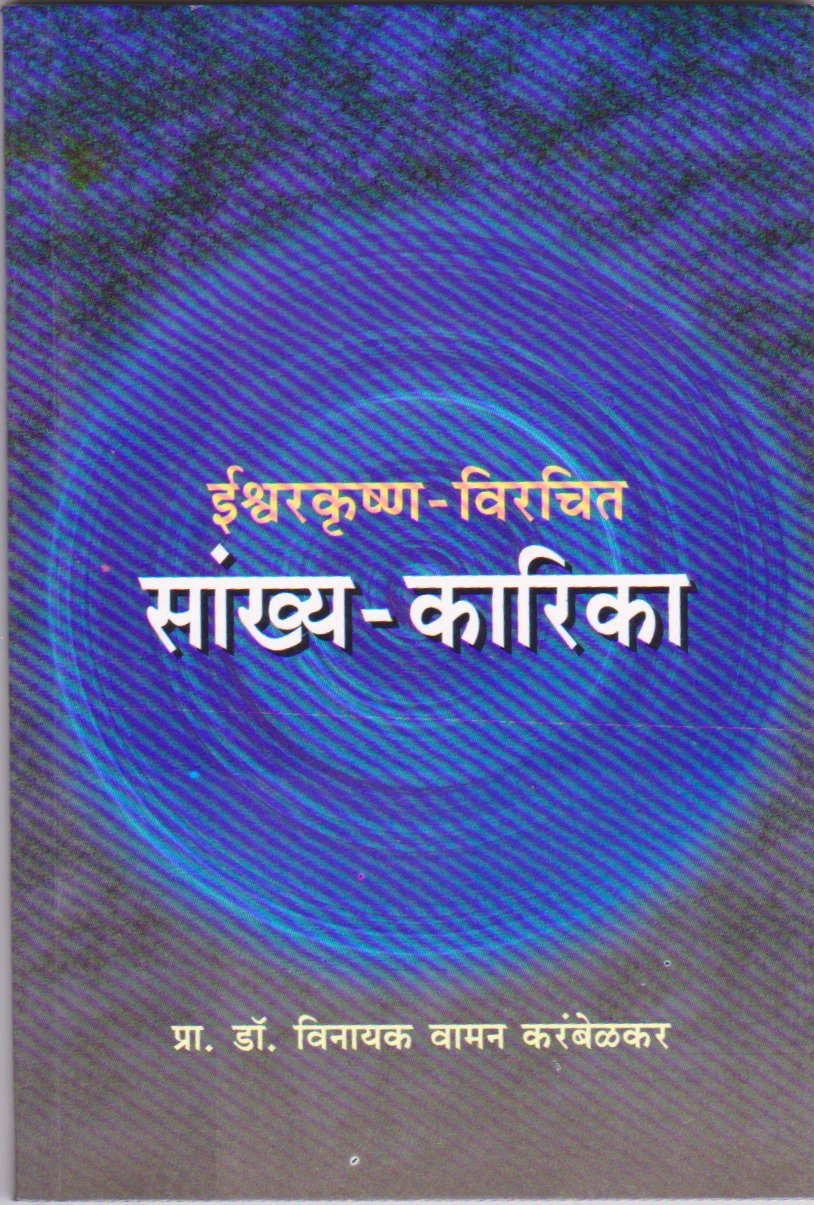
\includegraphics[width=\linewidth,keepaspectratio]{sankhya3}
      \end{center}	
    \end{column}
\end{columns}
\end{frame}

%%%%%%%%%%%%%%%%%%%%%%%%%%%%%%%%%%%%%%%%%%%%%%%%%%%%%%%%%%%%%%%%%%%%%%%%%%%%%%%%%%
\begin{frame}[fragile]\frametitle{सत्कार्यवाद (Satkāryavāda)}
\begin{columns}
    \begin{column}[T]{0.6\linewidth}
      \begin{itemize}
		\item सत कर्म से ही सत कार्य उत्पन्न होते हैं ऐसा नहीं की असत से सत नहीं बन सकता है 
		\item आप यह नहीं का सकते की कुछ नहीं था और उससे कुछ बन गया
        \item कारण (cause) में कार्य (effect) की पूर्वस्थिति होती है. For effect there has to be a cause.
        \item \textbf{सत् (Sat)} से ही \textbf{सत्कार्य (Satkārya)} उत्पन्न होता है
        \item "शून्य से कुछ नहीं बनता" — \textbf{असत्कार्यवाद} का खंडन
        \item उदाहरण: बीज में वृक्ष की संभावना
        \item कार्य, कारण का दृश्य रूप है, कारण can be invisible, say, a thought.
        \item कारण के दो प्रकार: \textbf{निमित्त} (Nimitta) और \textbf{उपादान} (Upādāna)

      \end{itemize}
    \end{column}
    \begin{column}[T]{0.4\linewidth}
      \begin{center}
        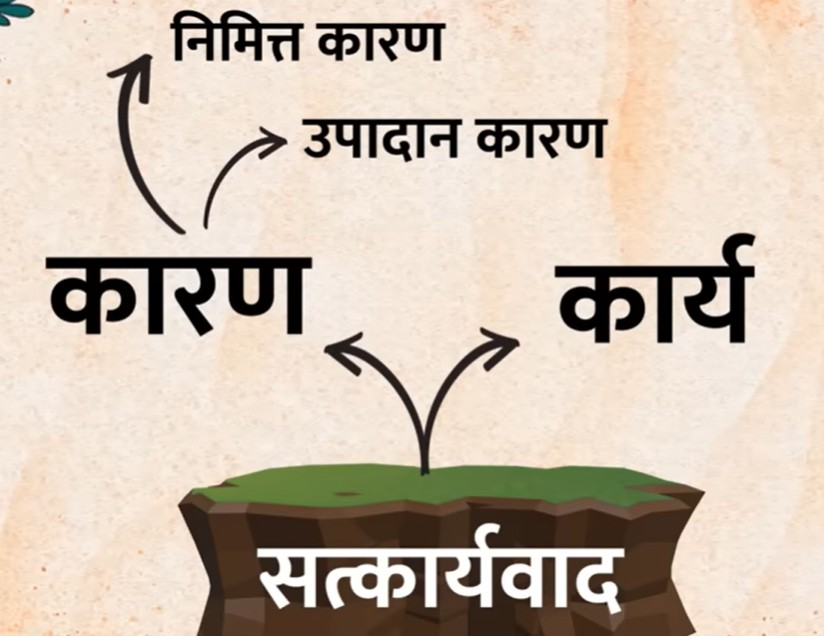
\includegraphics[width=\linewidth,keepaspectratio]{sankhya4}
		
		घड़े के लिए मिट्टी उपादान, कुम्हार निमित्त
		
        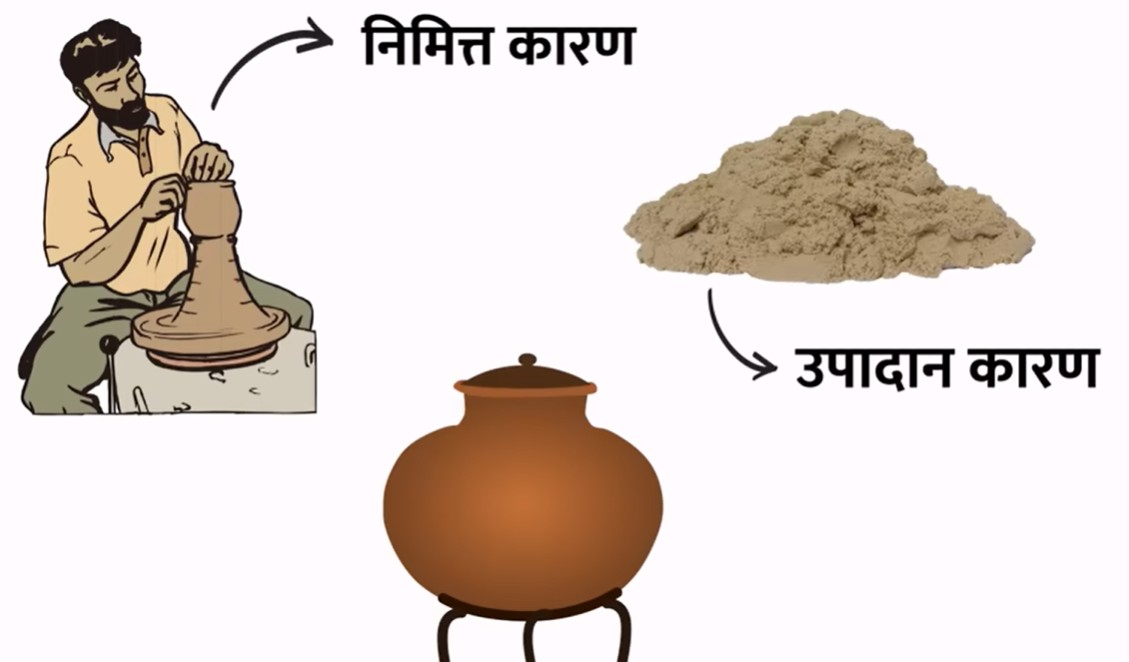
\includegraphics[width=\linewidth,keepaspectratio]{sankhya5}
		
		{\tiny (Ref: Samkhya Darshan - HyperQuest)}
		
      \end{center}	
    \end{column}
\end{columns}
\end{frame}

%%%%%%%%%%%%%%%%%%%%%%%%%%%%%%%%%%%%%%%%%%%%%%%%%%%%%%%%%%%%%%%%%%%%%%%%%%%%%%%%%%
\begin{frame}[fragile]\frametitle{ब्रह्मांड}

      \begin{itemize}
		\item ईश्वर (निमित्त) ने ब्रह्मांड को बनाया है लेकिन उपादान कारण क्या है? मिट्टी कहां से आई जो घड़ा बना उसके लिए ? 
		\item भगवान हो या ना हो लेकिन उपादान कारण तो चाहिए तो इसलिए उपादान कारण को फिर खोजना है. 
		\item हमारे पास कार्य हो कारण पता ही ना हो जैसे ये ब्रह्मांड कार्य तो हमें पता है की ब्रह्मांड बन गया है लेकिन कारण नहीं पता. संख्या दर्शन ये बोलता है की अगर हमारे पास कार्य है तो कार्य को देख कर कारण का अनुमान लगाया जा सकता है 
		\item जैसे की बच्चेको देखकर उसकेमातापिता कैसे होंगे यह अनुमान लगाया जा सकता है. या फिर ढेर सारे जोडे को खड़ा कर दिया जाए तो कुछ हद तक यह बताया जा सकता है की वो किसका बेटा है 
      \end{itemize}


\end{frame}

%%%%%%%%%%%%%%%%%%%%%%%%%%%%%%%%%%%%%%%%%%%%%%%%%%%%%%%%%%%%%%%%%%%%%%%%%%%%%%%%%%
\begin{frame}[fragile]\frametitle{ब्रह्मांड}

      \begin{itemize}
		\item आपके पास घडा है और आपके हाथ में बहुत ढेर सारे अलग-अलग तरह के पदार्थ दे दिए जाए तो आप ये तो नहीं बोलोगे की यह धर्म मोम का बना होगा मिट्टी जैसा रेट जैसा कुछ दिखेगा तो आप उसको बता सकते हो.
		\item ``ब्रह्मांड हमारे पास है है तो इसका कारण भी ब्रह्मांड जैसा होना चाहिए ''
      \end{itemize}

      \begin{center}
	
        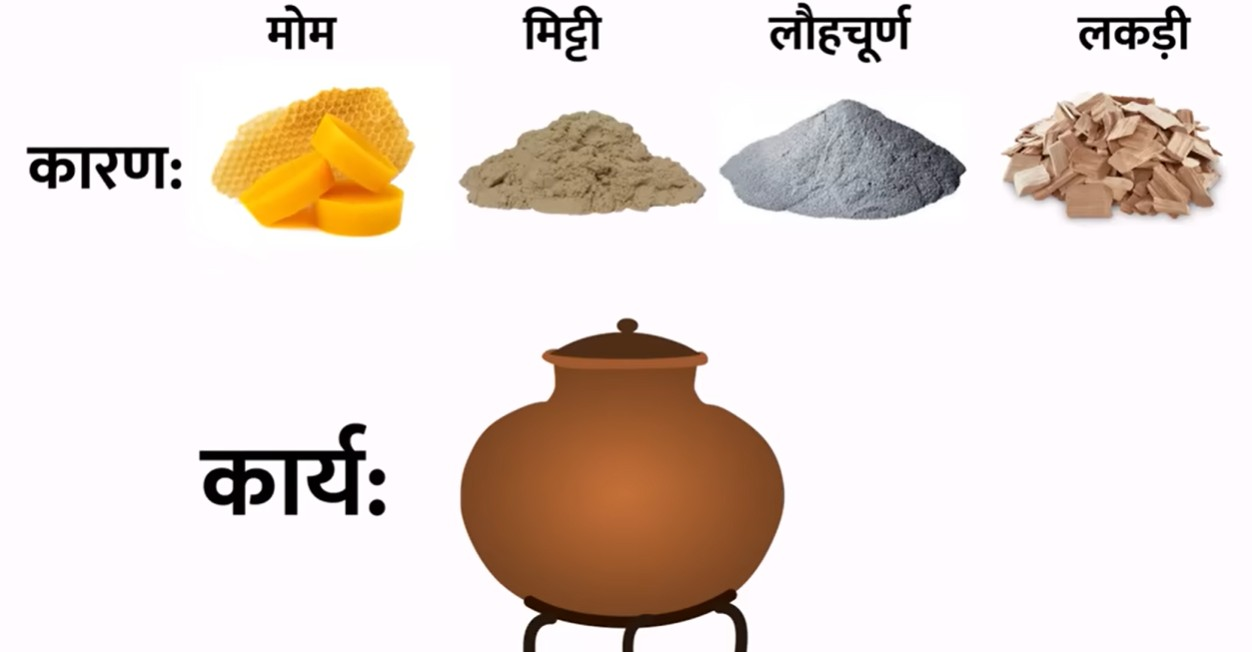
\includegraphics[width=0.8\linewidth,keepaspectratio]{sankhya6}
		
		{\tiny (Ref: Samkhya Darshan - HyperQuest)}
		
      \end{center}	
\end{frame}


%%%%%%%%%%%%%%%%%%%%%%%%%%%%%%%%%%%%%%%%%%%%%%%%%%%%%%%%%%%%%%%%%%%%%%%%%%%%%%%%%%
\begin{frame}[fragile]\frametitle{ब्रह्मांड}

      \begin{itemize}
		\item  ब्रह्मांड में तीन चीज प्रमुखता से दिखती 
		\item बहुत सी चीज प्रकाश वहां है प्रकाशित हैं बहुत तेजस्वी हैं और बहुत ढेर सारी चीज गतिमान है और तीसरी चीज की बहुत सी चीज
अंधेरे में है तो ये तीन तरह के उनको निरीक्षण दिखते हैं ब्रह्मांड में 
		\item पृथ्वी पर भी निरीक्षण करते हैं तो कुछ इंसान जो है बहुत सुखी दिखते हैं उनके चेहरे पे तेज दिखता है कुछ इंसान भागदौड़ी में है लेकिन बहुत पेन में है पीड़ा में है दुखी हैं और कुछ इंसान एकदम ही आलसी हैं मतलब उदासीन है जैसे लगता है जीवन में फंसे हुए हैं 
		\item तो ये तीन तरह की चीज ब्रह्मांड में हमारे ऋषि मुनियों को दिखी तो उन्होंने ये माना की जब ब्रह्मांड में कार्य में ये तीन इफेक्ट है यह तीन तरह के गुण है तो उसके कारण में भी ये तीन गुण होने चाहिए तभी उससे ये ब्रह्मांड आ  सकता है अगर कारण में तीन गुण नहीं है तो कार्य
में भी ये तीन गुण नहीं होंगे 
		\item सांख्य दर्शन ने ब्रह्मांड का जो उपादान कारण है उसको प्रकृति माना
		\item प्रकृति मतलब प्र+कृति, कृति मतलब कार्य,  प्रा-> पहले. तो कार्य से पहले जो कारण आया है ब्रह्मांड का उसको प्रकृति
बोला
      \end{itemize}

\end{frame}


%%%%%%%%%%%%%%%%%%%%%%%%%%%%%%%%%%%%%%%%%%%%%%%%%%%%%%%%%%%%%%%%%%%%%%%%%%%%%%%%%%
\begin{frame}[fragile]\frametitle{प्रकृति – उपादान कारण (Prakṛti as Material Cause)}

      \begin{itemize}
        \item ब्रह्मांड का उपादान कारण: \textbf{प्रकृति (Prakṛti)},         प्रकृति = \textbf{प्रधान} = मूल कार्य (ब्रह्मांड) का स्रोत. \textbf{अव्यक्त} (Avyakta), \textbf{अज} (Unborn), \textbf{अनादि} (Eternal)
        \item प्रकृति त्रिगुणात्मक: \textbf{सत्त्व}, \textbf{रजस्}, \textbf{तमस्}, सत्त्व – प्रकाश, रजस् – गति, तमस् – आलस 
		\item प्रकृति तो बहुत असीम माना गया है लेकिन असीम मरने के साथ-साथ उसको जड़ माना गया की उसमें बुद्धि नहीं है वो खुद से नहीं बना सकती 
		\item कौन से गुण किस अनुपात में मिल के सत रज  तम का कौन-कौन सा किस अनुपात से मिलकर यह ब्रह्मांड बने गए
ब्रह्मांड की कौन सी चीज कितने अनुपात में बनेगी ये प्रकृति के बस का नहीं है क्योंकि उसके पास खुद की चेतना नहीं है वो जड़ है 
        \item प्रकृति जड़ (बुद्धिहीन ) है, चेतना नहीं रखती. मूल प्रकृति बस आइडिया है वह अव्यक्त है 
        \item जब साम्यावस्था भंग होती है, तभी सृष्टि प्रारंभ
		\item सांख्य दर्शन बोलता है पुरुष जो ये चेतना है  
	
      \end{itemize}

\end{frame}

%%%%%%%%%%%%%%%%%%%%%%%%%%%%%%%%%%%%%%%%%%%%%%%%%%%%%%%%%%%%%%%%%%%%%%%%%%%%%%%%%%
\begin{frame}[fragile]\frametitle{पुरुष – चेतन तत्त्व (Puruṣa – Conscious Principle)}
सांख्य दर्शन को द्वैतवाद बोलते हैं की दो प्रमुख मूल तत्व हैं एक है प्रकृति जो कारण है उपादान कारण है जिससे ब्रह्मांड बना है और फिर उसे
प्रकृति में चूंकि जड़ता है उसके पास खुद का दिमाग नहीं है वो बस साम्यावस्था में है उसके पास तीन गुण इसलिए हैं क्योंकि ब्रह्मांड में भी तीन गुण देखते हैं यह तीन गुण कैसे मिलके ब्रह्मांड बनेगा इसके लिए चाहिए चेतना और उसे चेतना को फिर पुरुष बोला अब प्रकृति और पुरुष समीप आते हैं उनसे ब्रह्मांड कैसे बनता है

\begin{columns}
    \begin{column}[T]{0.5\linewidth}
      \begin{itemize}
        \item \textbf{पुरुष (Puruṣa)} – शुद्ध चेतना
        \item अनुभव करने वाला, किन्तु कर्ता नहीं
        \item \textbf{निर्गुण}, \textbf{अक्रिय}, \textbf{साक्षी रूप}
        \item अनेक पुरुष – हर जीव में एक चेतना
        \item प्रकृति और पुरुष के संयोग से सृष्टि आरंभ होती है
        \item पुरुष का उद्देश्य – केवल \textbf{दर्शन} और \textbf{अनुभव}
        \item पुरुष दुख के कारण नहीं, मात्र दर्शक है
      \end{itemize}
    \end{column}
    \begin{column}[T]{0.5\linewidth}
      \begin{center}
        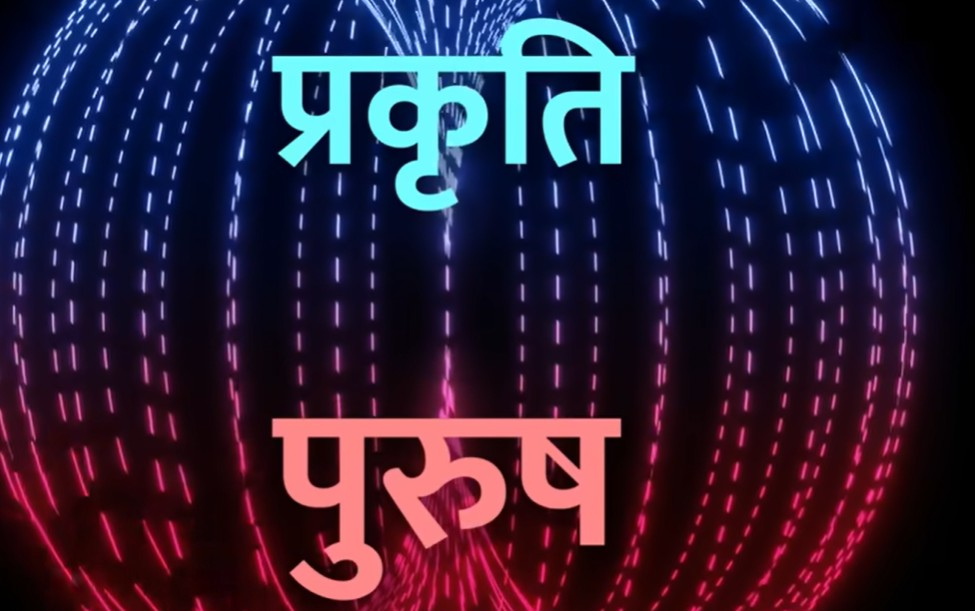
\includegraphics[width=\linewidth,keepaspectratio]{sankhya7}
      \end{center}	
    \end{column}
\end{columns}
\end{frame}

% %%%%%%%%%%%%%%%%%%%%%%%%%%%%%%%%%%%%%%%%%%%%%%%%%%%%%%%%%%%%%%%%%%%%%%%%%%%%%%%%%%
% \begin{frame}[fragile]\frametitle{२५ तत्त्व (25 Tattvas in Sāṅkhya)}
% \begin{columns}
    % \begin{column}[T]{0.6\linewidth}
      % \begin{itemize}
        % \item 1. \textbf{प्रकृति (Prakṛti)}
        % \item 2. \textbf{महत्/बुद्धि (Mahad/Buddhi)}
        % \item 3. \textbf{अहंकार (Ahaṃkāra)}
        % \item 4–8. \textbf{पञ्च तन्मात्राएँ (Tanmātrā)} – रूप, रस, गंध, स्पर्श, शब्द
        % \item 9–13. \textbf{पञ्च महाभूत} – पृथ्वी, जल, अग्नि, वायु, आकाश
        % \item 14–18. \textbf{पञ्च ज्ञानेंद्रियाँ} – आँख, कान, नाक, जीभ, त्वचा
        % \item 19–23. \textbf{पञ्च कर्मेंद्रियाँ} – हाथ, पैर, वाणी, मल, उपस्थ
        % \item 24. \textbf{मनः (Manas)}
        % \item 25. \textbf{पुरुष (Puruṣa)}
      % \end{itemize}
    % \end{column}
    % \begin{column}[T]{0.4\linewidth}
      % \begin{center}
        % \includegraphics[width=0.8\linewidth,keepaspectratio]{25_tattva}
      % \end{center}	
    % \end{column}
% \end{columns}
% \end{frame}

% %%%%%%%%%%%%%%%%%%%%%%%%%%%%%%%%%%%%%%%%%%%%%%%%%%%%%%%%%%%%%%%%%%%%%%%%%%%%%%%%%%
% \begin{frame}[fragile]\frametitle{दुःख का स्वरूप (Nature of Duḥkha)}
% \begin{columns}
    % \begin{column}[T]{0.6\linewidth}
      % \begin{itemize}
        % \item जीवन का मूल उद्देश्य – \textbf{दुःख से निवृत्ति}
        % \item तीन प्रकार के दुःख (त्रिताप) —
          % \begin{itemize}
            % \item \textbf{आधिभौतिक (Ādhibhautika)} – शरीर/प्रकृति से
            % \item \textbf{आधिदैविक (Ādhidaivika)} – प्राकृतिक आपदाएँ आदि
            % \item \textbf{आध्यात्मिक (Ādhyātmika)} – मानसिक/आत्मिक पीड़ा
          % \end{itemize}
        % \item सुख अल्पकालिक, दुःख सर्वत्र
        % \item दुःख की जड़ – प्रकृति से असम्यक् संयोग
        % \item \textbf{विवेकज्ञान} (discriminative knowledge) से मुक्ति संभव
      % \end{itemize}
    % \end{column}
    % \begin{column}[T]{0.4\linewidth}
      % \begin{center}
        % \includegraphics[width=0.8\linewidth,keepaspectratio]{duhkha_types}
      % \end{center}
    % \end{column}
% \end{columns}
% \end{frame}

% %%%%%%%%%%%%%%%%%%%%%%%%%%%%%%%%%%%%%%%%%%%%%%%%%%%%%%%%%%%%%%%%%%%%%%%%%%%%%%%%%%
% \begin{frame}[fragile]\frametitle{मोक्ष – कैवल्य (Liberation as Kaivalya)}
% \begin{columns}
    % \begin{column}[T]{0.6\linewidth}
      % \begin{itemize}
        % \item \textbf{मोक्ष = कैवल्य} – पुरुष की पूर्ण स्वतंत्रता
        % \item पुरुष और प्रकृति का भेदज्ञान होने पर \textbf{विवेक} उत्पन्न होता है
        % \item प्रकृति पुरुष के लिए अनुभव कराती है, फिर निवृत्त हो जाती है
        % \item कैवल्य – न दुःख, न सुख, केवल शुद्ध साक्षित्व
        % \item \textbf{न आत्मा का विलय}, न ब्रह्म में लय – पुरुष सदा स्वतंत्र
        % \item मुक्त पुरुष के लिए सृष्टि नहीं रह जाती
        % \item मोक्ष के बाद शरीर रहने पर भी मन/बुद्धि निष्क्रिय
      % \end{itemize}
    % \end{column}
    % \begin{column}[T]{0.4\linewidth}
      % \begin{center}
        % \includegraphics[width=0.8\linewidth,keepaspectratio]{kaivalya}
      % \end{center}
    % \end{column}
% \end{columns}
% \end{frame}


% %%%%%%%%%%%%%%%%%%%%%%%%%%%%%%%%%%%%%%%%%%%%%%%%%%%%%%%%%%%%%%%%%%%%%%%%%%%%%%%%%%
% \begin{frame}[fragile]\frametitle{त्रिगुण – प्रकृति की तीन धाराएँ (Three Guṇas of Prakṛti)}
% \begin{columns}
    % \begin{column}[T]{0.6\linewidth}
      % \begin{itemize}
        % \item प्रकृति की मूल प्रवृत्तियाँ: \textbf{सत्त्व}, \textbf{रजस्}, \textbf{तमस्}
        % \item \textbf{सत्त्व (Sattva)} – शुद्धता, ज्ञान, संतुलन, प्रकाश
        % \item \textbf{रजस् (Rajas)} – क्रिया, गति, इच्छा, उतेजना
        % \item \textbf{तमस् (Tamas)} – जड़ता, मोह, आलस्य, अज्ञान
        % \item ये तीनों एक-दूसरे पर प्रभाव डालते हैं – कभी कोई एक प्रबल होता है
        % \item व्यक्तित्व, मनोदशा, व्यवहार इन गुणों के मिश्रण पर निर्भर
        % \item मोक्ष हेतु सत्त्व की प्रधानता आवश्यक
      % \end{itemize}
    % \end{column}
    % \begin{column}[T]{0.4\linewidth}
      % \begin{center}
        % \includegraphics[width=0.8\linewidth]{triguna_chart}
      % \end{center}
    % \end{column}
% \end{columns}
% \end{frame}

% %%%%%%%%%%%%%%%%%%%%%%%%%%%%%%%%%%%%%%%%%%%%%%%%%%%%%%%%%%%%%%%%%%%%%%%%%%%%%%%%%%
% \begin{frame}[fragile]\frametitle{अहंकार – कर्तृत्व की भावना (Ahaṃkāra – Sense of 'I')}
% \begin{columns}
    % \begin{column}[T]{0.6\linewidth}
      % \begin{itemize}
        % \item \textbf{महत्} (बुद्धि) से उत्पन्न होता है \textbf{अहंकार}
        % \item “मैं करता हूँ” की धारणा – आत्म-बोध का भ्रम
        % \item त्रिगुणों के अनुसार तीन प्रकार:
          % \begin{itemize}
            % \item \textbf{सात्त्विक} – ज्ञानेंद्रियाँ, मन
            % \item \textbf{राजसिक} – कर्मेंद्रियाँ
            % \item \textbf{तामसिक} – तन्मात्राएँ, महाभूत
          % \end{itemize}
        % \item अहंकार के बिना "स्व" का भ्रम नहीं उत्पन्न होता
        % \item मोक्ष हेतु अहंकार का लय आवश्यक
      % \end{itemize}
    % \end{column}
    % \begin{column}[T]{0.4\linewidth}
      % \begin{center}
        % \includegraphics[width=0.8\linewidth]{ahamkara_tree}
      % \end{center}
    % \end{column}
% \end{columns}
% \end{frame}

% %%%%%%%%%%%%%%%%%%%%%%%%%%%%%%%%%%%%%%%%%%%%%%%%%%%%%%%%%%%%%%%%%%%%%%%%%%%%%%%%%%
% \begin{frame}[fragile]\frametitle{मन, बुद्धि, चित्त – अंतर व संबंध (Mind, Intellect, and Memory)}
% \begin{itemize}
  % \item \textbf{बुद्धि (Buddhi)} – निर्णय करने की शक्ति, विवेक-तत्त्व
  % \item \textbf{अहंकार (Ahaṃkāra)} – ‘मैं’ और ‘मेरा’ की भावना
  % \item \textbf{मन (Manas)} – इंद्रियों से सूचना ग्रहण व संचालन
  % \item \textbf{चित्त (Citta)} – स्मृति, संस्कार, मनोवृत्तियाँ
  % \item चारों \textbf{अंतःकरण चतुष्टय} कहलाते हैं
  % \item सांख्य में चित्त का पृथक उल्लेख नहीं – बुद्धि के रूप में ही मानते हैं
  % \item योग दर्शन चित्त को स्वतंत्र रूप से मानता है
% \end{itemize}
% \end{frame}


% %%%%%%%%%%%%%%%%%%%%%%%%%%%%%%%%%%%%%%%%%%%%%%%%%%%%%%%%%%%%%%%%%%%%%%%%%%%%%%%%%%
% \begin{frame}[fragile]\frametitle{अन्य दर्शनों से तुलना (Comparison with Other Darśanas)}
% \begin{itemize}
  % \item \textbf{योग दर्शन} – सांख्य दर्शन का व्यावहारिक अनुप्रयोग
  % \item \textbf{वेदांत} – ब्रह्म एक, अद्वैत; सांख्य – द्वैत (प्रकृति+पुरुष)
  % \item \textbf{बौद्ध} – अनात्मवाद; सांख्य – अनेक आत्माएँ (पुरुष)
  % \item \textbf{न्याय-वैशेषिक} – तर्क और पदार्थ के आधार पर सृष्टि; सांख्य – विवेक व प्रकृति के आधार पर
  % \item \textbf{जैन दर्शन} – आत्मा और द्रव्य अलग, कर्म बंधन से मुक्ति; सांख्य – प्रकृति से भेद ही मुक्ति
  % \item सांख्य – सर्वप्रथम \textbf{अनुभववाद + विश्लेषण} का प्रयोग
% \end{itemize}
% \end{frame}

% %%%%%%%%%%%%%%%%%%%%%%%%%%%%%%%%%%%%%%%%%%%%%%%%%%%%%%%%%%%%%%%%%%%%%%%%%%%%%%%%%%
% \begin{frame}[fragile]\frametitle{योग दर्शन से संबंध (Relation with Yoga Philosophy)}
% \begin{itemize}
  % \item योग दर्शन सांख्य का ही व्यावहारिक रूप है
  % \item \textbf{पतंजलि योगसूत्र} में सांख्य के सिद्धांत आधार हैं
  % \item सांख्य – सिद्धांत; योग – अनुशासन, अभ्यास
  % \item योग में चित्तवृत्तियों का निरोध; सांख्य में विवेक का विकास
  % \item दोनों का लक्ष्य – \textbf{कैवल्य} / मोक्ष
  % \item सांख्य दर्शन ईश्वर को स्वीकार नहीं करता; योग दर्शन \textbf{ईश्वरप्रणिधान} को स्थान देता है
  % \item दोनों में 25 तत्त्वों की स्वीकृति समान
% \end{itemize}
% \end{frame}

% %%%%%%%%%%%%%%%%%%%%%%%%%%%%%%%%%%%%%%%%%%%%%%%%%%%%%%%%%%%%%%%%%%%%%%%%%%%%%%%%%%
% \begin{frame}[fragile]\frametitle{वैज्ञानिक दृष्टिकोण (Scientific Outlook)}
% \begin{itemize}
  % \item सांख्य दर्शन का विश्लेषणात्मक दृष्टिकोण आधुनिक विज्ञान से मेल खाता है
  % \item \textbf{सत्कार्यवाद} = ऊर्जा/पदार्थ के संरक्षण का सिद्धांत
  % \item \textbf{त्रिगुण सिद्धांत} – मनोविज्ञान और न्यूरोसाइंस से संबंधित
  % \item \textbf{25 तत्त्व} – एक प्रकार की सांख्यिकी (taxonomy) है
  % \item \textbf{निष्क्रिय पुरुष, सक्रिय प्रकृति} – ऑब्जर्वर थेओरी (Observer Effect)
  % \item \textbf{विवेकज्ञान} = मेटा-कॉग्निशन (Self-awareness)
  % \item भौतिक और मानसिक दोनों जगत का संतुलित विश्लेषण
% \end{itemize}
% \end{frame}

% %%%%%%%%%%%%%%%%%%%%%%%%%%%%%%%%%%%%%%%%%%%%%%%%%%%%%%%%%%%%%%%%%%%%%%%%%%%%%%%%%%
% \begin{frame}[fragile]\frametitle{समकालीन उपयोगिता (Modern Relevance)}
% \begin{itemize}
  % \item मानसिक स्वास्थ्य में त्रिगुण सिद्धांत का प्रयोग
  % \item आत्मनिरीक्षण और mindfulness के आधार पर विवेक
  % \item योग और ध्यान में सांख्य दर्शन का मूल आधार
  % \item विज्ञान, मनोविज्ञान, न्यूरोलॉजी में उपयोगी दृष्टिकोण
  % \item दार्शनिक अध्ययन में द्वैतवाद की बुनियाद
  % \item नैतिकता व मोक्ष की व्यक्तिगत समझ को प्रोत्साहन
% \end{itemize}
% \end{frame}

% %%%%%%%%%%%%%%%%%%%%%%%%%%%%%%%%%%%%%%%%%%%%%%%%%%%%%%%%%%%%%%%%%%%%%%%%%%%%%%%%%%
% \begin{frame}[fragile]\frametitle{निष्कर्ष – सांख्य दर्शन का सार (Conclusion)}
% \begin{itemize}
  % \item दो स्वतंत्र तत्त्व – \textbf{प्रकृति} और \textbf{पुरुष}
  % \item सृष्टि – प्रकृति द्वारा पुरुष के लिए अनुभव का माध्यम
  % \item त्रिगुणों के संयोग से विविध रूपों की उत्पत्ति
  % \item दुःख – अविवेक से उत्पन्न; मोक्ष – विवेक से
  % \item मोक्ष का अर्थ – प्रकृति से पुरुष का पूर्ण वैराग्य
  % \item अत्यंत तर्कसंगत, विज्ञानसम्मत एवं अनुभवशील दर्शन
  % \item योग, वेदांत, आधुनिक विज्ञान सभी पर प्रभाव
% \end{itemize}
% \end{frame}

%%%%%%%%%%%%%%%%%%%%%%%%%%%%%%%%%%%%%%%%%%%%%%%%%%%%%%%%%%%%%%%%%%%%%%%%%%%%%%%%%%
\begin{frame}[fragile]\frametitle{References}

      \begin{itemize}
        \item Samkhya Darshan - HyperQuest
      \end{itemize}

\end{frame}


